% **************************************************
% Document Class Definition
% **************************************************
\documentclass[%
	paper=A4,					% paper size --> A4 is default in Germany
	twoside=true,				% onesite or twoside printing
	openright,					% doublepage cleaning ends up right side
	parskip=full,				% spacing value / method for paragraphs
	chapterprefix=true,			% prefix for chapter marks
	11pt,						% font size
	headings=normal,			% size of headings
	bibliography=totoc,			% include bib in toc
	listof=totoc,				% include listof entries in toc
	titlepage=on,				% own page for each title page
	captions=tableabove,		% display table captions above the float env
	draft=true,				% value for draft version
]{scrreprt}%

% **************************************************
% Debug LaTeX Information
% **************************************************
%\listfiles

% **************************************************
% Information and Commands for Reuse
% **************************************************
\newcommand{\thesisTitle}{Mixed Reality Media: Integration of live video feed in 3D environments}
\newcommand{\thesisName}{Martin Zier}
\newcommand{\thesisSubject}{Bachelor Thesis}
\newcommand{\thesisDate}{\today}
\newcommand{\thesisVersion}{Initial Drafting}

\newcommand{\thesisFirstReviewer}{Kristian Hildebrand}
\newcommand{\thesisFirstReviewerUniversity}{\protect{Beuth University of Applied Sciences}}
\newcommand{\thesisFirstReviewerDepartment}{Department VI: Computer Sciences and Media}

\newcommand{\thesisSecondReviewer}{Prof. Dr.-Ing. Ren\'e G\"orlich}
\newcommand{\thesisSecondReviewerUniversity}{\protect{Beuth University of Applied Sciences}}
\newcommand{\thesisSecondReviewerDepartment}{Department VI: Computer Sciences and Media}

\newcommand{\thesisFirstSupervisor}{Kristian Hildebrand}
\newcommand{\thesisSecondSupervisor}{Joachim Quantz}

\newcommand{\thesisUniversity}{\protect{Beuth University of Applied Sciences}}
\newcommand{\thesisUniversityDepartment}{Department VI: Computer Sciences and Media}
\newcommand{\thesisUniversityInstitute}{ }
\newcommand{\thesisUniversityGroup}{ }
\newcommand{\thesisUniversityCity}{Berlin}
\newcommand{\thesisUniversityStreetAddress}{Luxemburger Stra{\ss}e 10}
\newcommand{\thesisUniversityPostalCode}{13353}

% **************************************************
% Load and Configure Packages
% **************************************************
\usepackage[utf8]{inputenc}		% defines file's character encoding
\usepackage[english]{babel} % babel system, adjust the language of the content
\usepackage[					% clean thesis style
	figuresep=colon,%
	sansserif=false,%
	hangfigurecaption=false,%
	hangsection=true,%
	hangsubsection=true,%
	colorize=full,%
	colortheme=bluemagenta,%
	bibsys=bibtex,%
	bibfile=bib-refs,%
	bibstyle=alphabetic,%
]{cleanthesis}

\usepackage{todonotes}
\usepackage{listings}
\usepackage{amsmath}
\usepackage{mathtools}
\usepackage{subcaption}
\usepackage{cleveref}
\usepackage[toc]{appendix}


\hypersetup{					% setup the hyperref-package options
	pdftitle={\thesisTitle},	% 	- title (PDF meta)
	pdfsubject={\thesisSubject},% 	- subject (PDF meta)
	pdfauthor={\thesisName},	% 	- author (PDF meta)
	plainpages=false,			% 	-
	colorlinks=false,			% 	- colorize links?
	pdfborder={0 0 0},			% 	-
	breaklinks=true,			% 	- allow line break inside links
	bookmarksnumbered=true,		%
	bookmarksopen=true			%
}

% Glossaries needs to be after hyperref to enable linking.
\usepackage[toc]{glossaries} 

\makeglossaries
% !TeX spellcheck = en_US
% !TEX root = ../thesis-example.tex
%

\newglossaryentry{computer}{
	name={computer},
	description={we tricked a rock into thinking by putting lightning into it.},
	plural={computers}}

\newglossaryentry{framebuffer}{
	name={framebuffer},
	description={It usually contains ARGB data of each remaining fragment. It 
	can, however, contain any form of data, including fragment vector depth, 
	depth-normals, normals and so on.},
	plural={framebuffers}
}

\newglossaryentry{render texture}{
	name={RenderTexture},
	description={Unity exposes frame buffers as render textures. It is not 
	possible to access both dat and depth buffer on one frame buffer, which can 
	be circumvented by seperate RenderTextures with no data or depth buffer.}
}

\newglossaryentry{fragment}{
	name={Fragment},
	description={It is a rasterized pixel of a vertex (usually a triangle).}
	plural={fragments}
}

\newglossaryentry{head mounted display}{
	name={Head Mounted Display},
	description={A general term for display solutions mounting on the users 
	head. Recent examples with spatial tracking are HTC Vive, Oculus Rift and 
	Microsoft HoloLens. Untracked examples are Google Glasses or to an extend 
	Google Cardboard.},
	plural={Head Mounted Displays}
}

\newglossaryentry{6dofg}{
	name={6DOF},
	description={Describes free movement of a rigid body in 
		three-dimensional space - specifically forward/backward (surge), 
		up/down (heave), left/right (sway) translations, combined with changed 
		of rotations around all three axis. \textbf{may need wikipedia cite}
	}
}

\newglossaryentry{6dof}{
	type=\acronymtype,
	name={6DOF},
	description={Six Degrees of Freedom (6DOF) \glsadd{6dofg}},
	see=[Glossary:]{6dofg}
}

\newacronym{6DOF}{6DOF}{Six Degrees of Freedom}

\newacronym[longplural={Frames per Second}]{acr:fps}{fps}{frames per second} % actually is a glossary, sorry.

% **************************************************
% Document CONTENT
% **************************************************
\begin{document}

% --------------------------
% rename document parts
% --------------------------
%\renewcaptionname{ngerman}{\figurename}{Abb.}
%\renewcaptionname{ngerman}{\tablename}{Tab.}
\renewcaptionname{english}{\figurename}{Fig.}
\renewcaptionname{english}{\tablename}{Tab.}

% --------------------------
% Front matter
% --------------------------
\pagenumbering{roman}			% roman page numbing (invisible for empty page style)
\pagestyle{empty}				% no header or footers
\input{content/titlepages}		% INCLUDE: all titlepages
\cleardoublepage

\pagestyle{plain}				% display just page numbers
% !TeX spellcheck = en_US
% !TEX root = ../thesis-example.tex
%
\pdfbookmark[0]{Abstract}{Abstract}
\chapter*{Abstract}
\label{sec:abstract}
\vspace*{-10mm}

Virtual Reality is no distance dream anymore, but the technology has a 
marketing problem: A view through the eyes of the head-mounted display wearer 
is bland and loses the usage context. Following the first-person view is hard 
and it shows twitchy, unnatural motion.

This thesis discusses a general rendering pipeline for runtime 3D engines for 
Mixed Reality Media, a form of video composition that places a real person 
inside a virtual reality scene. The real world video will be augmented by 
multiple video techniques and parameters from the virtual environment.
\newline
For example this allows for recreation of light conditions from the virtual 
scene and creates an immersive and inviting view into the virtual scenery.

\begin{center}
	\hrulefill
\end{center}

VR ist kein entfernter Traum mehr, doch die Technologie hat ein 
Marketing-Problem: Ein Blick durch die Augen des Headset-Trägers ist 
uninteressant und verliert den Nutzerkontext. Der First-Person Sicht ist nur 
schwer zu folgen und zeigt unruhige, unnatürliche Bewegungen.

Diese Bachelor Arbeit beschäftigt sich mit dem Aufbau einer allgemeinen Mixed 
Reality Pipeline für Echtzeit 3D Engines, eine Aufarbeitung von 
Echtbildaufnahmen eines VR Nutzers und die Rückführung in eine virtuelle Szene. 
Durch mehrere Videoverfahren wird das Bild des Trägers mit der virtuellen Welt 
zusammengeführt und mit den Parametern der virtuellen Welt erweitert.
\newline
Dadurch können z. B. Lichtverhältnisse der virtuellen Szenerie nachempfunden 
werden und einen immersiven und einladenden Blick in den virtuellen Raum 
geboten werden.		% INCLUDE: the abstracts (english and german)
\cleardoublepage
%
% !TeX spellcheck = en_US
% !TEX root = ../thesis-example.tex
%
\pdfbookmark[0]{Acknowledgement}{Acknowledgement}
\chapter*{Acknowledgement}
\label{sec:acknowledgement}
\vspace*{-10mm}

This thesis is dedicated to background noise: 

Background noise! Background noise makes nothing easier - get it now from your 
local certified background noise dealer.
 % INCLUDE: acknowledgement
\cleardoublepage
%
\setcounter{tocdepth}{2}		% define depth of toc
\tableofcontents				% display table of contents
\cleardoublepage

% --------------------------
% Body matter
% --------------------------
\pagenumbering{arabic}			% arabic page numbering
\setcounter{page}{1}			% set page counter
\pagestyle{maincontentstyle} 	% fancy header and footer

% !TEX root = ../thesis-example.tex
%
\chapter{Introduction}
\label{sec:intro}

\cleanchapterquote{If a technological feat is possible, man will do it. Almost 
as if it's wired into the core of our being.}{Motoko Kusanagi}{(Ghost in the 
Shell)}

Extending reality with the help of computer generated imagery is no new 
concept. Ever since real time 3D graphics was possible there was an attempt to 
extend the understanding of reality. Within the recent years there have been 
great successes in the industry, most notably in image augmentation was 
"Pok\'emon Go" with an estimated install base of 750 million downloads 
worldwide in June, 2017. \cite{appannie:2017}  Just before this thesis 
started, Apple and Google showed off their consumer-ready hard- and software 
for augmented reality experiences.
\newline
Virtual Reality Head Mounted Displays have had a similar push in sales with an 
approximate of 5.83 million sold devices, which range in a sales price between 
80 - 900€ for a VR kit, ranging from the very simple Google Daydream View and 
the very sophisticated HTC Vive. \cite{erguerel:2017} And in these figures are 
the sales of Google Cardboards missing, which is approximated at around 80 
Million.
\newline
This generation of computer systems, in which are PC workstations, game 
consoles and smartphones, is finally sophisticated enough in computation speed 
and sensor-sensitivity to allow low latency tracking, precise to just a few 
millimeters.

\section{Overview}
\label{sec:intro:outline}

The idea of Virtual Reality (VR) and Head Mounted Displays (HMDs) stems from a 
cultural need to switch into roles of foreign worlds. Through the advancing 
development of hard- and software over the last decades emerges a medium which 
has unmatched immersion and creates an unique, transforming experience into any 
imaginable environment.

VR and HMDs are now advanced enough for consumer markets - but it stumbles at 
communicating the experience. Without having ever put on a VR-Headset it is 
nearly impossible to understand - or even imagine - what the virtual reality 
experience means. Any observer of Virtual Reality, usually done by showing what 
the VR actor is seeing, will not be able to get an understand of the importance 
and shift of reality perception without wearing the headset himself.
\newline
Showing the video output from a HMD as marketing material is contradicting with 
classic motion video productions. There is even only one famous example where 
the perspective of a First Person Shooter is reenacted, which was in the 
overwhelmingly negatively received Doom (2005) movie.

The VR industry, including but not limited to game developers, exhibition 
creators and creative studios is in need of better communication of their 
products that includes more than the current headset wearer and allows for a 
similar, adapted and immersive experience.
\newline
The currently method is called "Mixed Reality" (MR) and uses an external camera 
with the same tracking hardware of the headset to produce a video signal that 
shows the real world actor with the environment around him. There are currently 
three main ways of producing MR footage - where as only one variant allows for 
live compositing with highly accurate imaging results.


\section{Motivation}
\label{sec:intro:motivation}

My early teenage years started around the time where digitalization and global
interconnectivity begun and broadband Internet became commercially available.
Suddenly remote multiplayer games, unlimited image sharing - and yes, music
sharing, too -, Java-Applets, Flash, HTML framesets and "Marquee" CSS emerged in
that medium. 3D Acceleration became a de-facto standard and even simple office
PCs got weak, but dedicated graphics processing units built in. The mass of
pixels by increasing the resolution of displays was basically a yearly
iteration in greater, better, smaller and brighter.

I am personally very interested and invested in Virtual/Mixed/Augmented Reality 
to succeed and liked the idea to merge multiple forms of media into one - which 
is, in my personal opinion, a great summary of my studies and its contents. 
This thesis represents my interests and the reasons why I chose these studies.

\section{Problem Statement}

Initially I will research motion video productions, computer generated imagery 
and color theory. This leads to the knowledge to implement basic, interactive 
live motion video.
\newline
The core aspect will be integrating a multitude of Hardware in a software that 
allows for dynamic video compositing in 3D environments at runtime while a user 
is interacting with the virtual reality scene. This allows that the person 
using the Vive HMD to be composited into the scenery and it looks like he is in 
that scene standing. The essential difference between classic post production 
is, that this system is planned to operate on runtime, allow additional 
observers to get an interesting composited imagery of what the VR actor is 
experiencing.
\newline
An additional extension is to dynamically track the camer position, allowing 
for dynamic camera movement and a freely moving actor. 
\section{Relevance \& Challenges}
\label{sec:intro:relevance}

\begin{my_list}
	\item Komplette Produktionsworkflow
	\item Chroma Keying
	\item Bildreproduktion
	\item Latencymitigation
	\item Tracking
\end{my_list}

Probably should be called Relevance \& Scope.

\section{Results}
\label{sec:intro:results}

Result stuff

\section{Thesis Structure}
\label{sec:intro:structure}

This thesis gets contemplated by digital, mostly motion video, material hosted 
on GitHub. Print is a great medium, but lacks the ability for short 
demonstrations of video imaging solutions, problems and edge cases. To 
visualize these problems properly, all video media will have an annotation for 
cross referencing on the website. It is strongly suggested to follow these 
links, they will be sorted by chapters.
% !TeX spellcheck = en_US
% !TEX root = ../thesis-example.tex
%
\chapter{Extending Reality}
\label{sec:extendingreality}

\cleanchapterquote{You are an aperture through which the universe is looking at 
and exploring itself.}{Alan W. Watts}{(Philosopher)}

The well known urban legend of "L'Arriv\'ee d'un train en gare de La Ciotat" in 
which a train arrives at the La Ciotat station, is, that "the audience was so 
overwhelmed by the moving image [...] coming directly at them that people 
screamed and ran to the back of the room". \cite{wiki:train:2017} With that a 
new medium was born, which matured into a new art form of film and movies.
\newline
Most important is that with this short clip opened a door beyond still images 
and their limited depiction of motion. Video imagery changed our imagination 
and allowed for a new communication form, inviting into an animated, moving 
world. There have been great achievements in the last century in motion video 
production with a great amount of visual trickery for composing more realistic 
and imaginative video content. With the help of Computer Generated Imagery 
(CGI) blurs the boundaries between real acting and virtual recreation so very 
far, that it is almost impossible to differentiate between real world video 
capture and 3D recreated imagery.

\section{Motion Video Production}

Producing motion video has come a long way and a sufficient history of it would 
be far out of scope for this thesis. Concentrating on key aspects of 
composition techniques might give an appropriate overview to range where Mixed 
Reality takes its inspiration from.

Way before digital imaging processing took over production sets similar 
problems as discussed in this thesis had to be solved, i. e. how an actor can 
be captured without a back- or foreground and how he would then be integrated 
into an imaginative set. Today, modern action movies don't even necessarily 
capture the actor but his movements, which then will be artificially rendered 
with computer generated imagery.

\todo[inline]{Missing: Camera tricks, computer aided visual effects, green 
screens}

\section{CGI \& Video Composition}

\subsection{History of Green \& Blue Screen Productions}

Set theory is beyond the scope of this thesis, but green- and blue screen 
production has first and foremost a simple reasoning: Green and blue are two of 
the three color triplets that resemble a least amount of color found in 
capturing of humans - and to a certain extent any flora and fauna. Since chroma 
keying (see Ch. \ref{sec:chromakey}) takes color distance as general basis, 
production environments generally use green screen keying.
\newline
Green boxes abuse a correlating advantage that the human eye is most 
susceptible to green, allowing for a visual high color range and an ability to 
differentiate between many shades of green. Experiments to color range have 
been done since 1942, trying to understand gambit ranges and color 
differentiation of human vision. Experiments concluded that eye cone cells see 
a blending range of wavelengths to different intensities, giving the green 
vector space its highest perceptible range. \cite{MacAdam:1942}

\begin{figure}[htbp]
	\label{fig:greenscreen:stimula}
	\begin{subfigure}[t]{.35\textwidth}
		\centering
		\includegraphics[width=\textwidth]{_external/media/CIExy1931_MacAdam.png}
	\caption{MacAdam ellipses on 1931 standard chromaticity diagram 
		\cite{wiki:macadam:2017}}
	\end{subfigure}
	\begin{subfigure}[t]{.5\textwidth}
		\centering
		\includegraphics[width=\textwidth]{_external/media/1280px-Cones_SMJ2_E.png}
		\caption{Normalized responsivity spectra of human cone cells, S, M, and 
		L types after Wyszecki et. al \cite{wiki:Wyszecki:2017}}. Notice the 
		overlap between M and L cones.
	\end{subfigure}
\end{figure}

\todo[inline]{The layout is a bit wonky here.}

Most consumer cameras - and even most production cameras - use dot-matrix 
sensors with a weighted ration of green (4), red (2) and blue (2) pixels, 
called Bayer pattern \cite{kodak:bayer:1976}. Green is generally easier to 
light, illuminate and adjust over blue screens. Small irregularities, for 
example through uneven lightning or crinkles in the material, can be adjusted 
easily by the user and allows for a relatively clean camera image generation.
\newline
The quality of input footage makes a big difference in separating back- and 
foreground, hence is a well lit and adjusted set a good backbone for well 
working chroma keying.

\section{What's VR - Differentiation of AR, VR \& MR}

In search of an appropriate abbreviation for computer-enhanced realtime imagery 
a recent addition is "XR", where \textit{X} is a letter of your choice. 
Definitions are getting more diluted and generally describe a technique, rather 
than an apparent effect by now.

\begin{figure}[htb]
	\includegraphics[width=\textwidth]{_raw_resources/i3-triangle.png}
	\caption{I\textsuperscript{3} Triangle - figurative quantization of 
		different reality extending methods}
	\label{fig:xr:i3-triangle}
\end{figure}
Augmented Reality (AR) is a concept by augmenting real world imagery with 
additional information and interactable objects. It ranges from very simple 
devices displaying data in the field of view of a user up to full augmentation, 
displaying 3D models overlaying on real world objects. This can be done ranging 
from Pepper's Ghost projections, augmenting video - a famous example is the 
rather successful "Pokémon GO" -, up to the Microsoft HoloLens, that has 
sensors for a wide range of spatial mapping, spatial anchoring and distance 
field calculation.

Virtual Reality is a concept usually done by stereo projection of a 3D 
environment inside a Head Mounted Display. It takes an user out of the current 
room and sets him into a complete new, virtual reality - hence it's names 
origin. HMD hardware ranges from the simplistic Google Cardboard 
\footnote{using a smartphone as display device} to the Samsung GearVR 
\footnote{similarly uses a smartphone as display driver} up to the Oculus Rift 
and HTC Vive. The latter two products offer room-scale experiences where a user 
is able to move freely in his play space (basically a tacked bounding volume) 
and allows for six degrees of freedom (\gls{6dof}) tracking.

Mixed Reality is an extension of Virtual Reality, allowing bystanders to get an 
impression of the virtual reality around an actor. By reproducing virtual 
projection parameters of a 3D environment, it is possible to place a real world 
camera feed at the right position inside the 3D application. This yields to a 
combined technique of Augmented and Virtual Reality. A production environment 
can be achieved with a \gls{6DOF} HMD and additional - either user- or tracking 
input of - positional parameters for the camera. 

\section{Immersion vs. Communication}

\todo[inline]{maybe the overview does already a "good enough" job to bring this 
across.}

Virtual Reality, as previously mentioned in \ref{sec:intro:outline}, is very 
immersive but the experience is hard to imagine without wearing a HMD yourself. 
Additionally doesn't VR offer any ways to allow observers a similar experience 
as the VR actor.
\newline
A very obvious problem starts on interaction. A VR user doesn't always need to 
see his hands to interact with a scene, due to the natural way of holding these 
controllers in his hands and directly translating controller interaction to the
virtual environment. An outside viewer however does not see hands and will 
not understand actions performed by the user if he cannot see the virtual 
hands. Any usage context that happens off-screen cannot be communicated and 
will be therefore lost.
\newline
A recent game example, Rick and Morty: Virtual Rick-ality, tries to mitigate 
this issue by placing virtual CCTV cameras into the scene, which can be 
controlled through outside viewers - giving a neutral third-person view into 
the three-dimension scene. The VR actor is replaced as a loose avatar 
representing a figure (Morty) from the cartoons universe.

\todo[inline]{Add a screenshot of that}

Mixed Reality merges the actors and virtual realities context, allowing outside 
bystanders a comparable window into the actors experienced world. In fact, 
initial promotional material for the HTC Vive showed mixed reality footage, 
produced by one VR computer and a secondary composition PC 
\cite{valve:mr-production:2016}. It's setup is comparable to the one in this 
thesis and differs by using more than one software context, done by outputting 
a rendered image of the virtual scene and compositing it on another system.

\subsection{Evolution of Virtual Reality Footage}

Originally footage consisted of the output that was sent to the headset, 
including image transformation that needs to be done to correct the headset 
lenses \footnote{this is referred to as "Barrel Distortion"} - this distorted 
dual image is very hard to follow, as it adds two ambiguous images and has 
additional a high distortion. Since the direct feed to a HMD is used, any 
translation of the headsets position is visible, which results in a jittery 
motion feed.

\begin{figure}[htbp]
	\label{fig:evolution:steps}
	\begin{subfigure}[t]{.45\textwidth}
		\centering
		\includegraphics[width=\textwidth]{_raw_resources/lens_distortion.jpeg}
		\caption{Distorted direct dual output to a Oculus DK2.}
	\end{subfigure}
	\begin{subfigure}[t]{.45\textwidth}
		\centering
		\includegraphics[width=\textwidth]{_raw_resources/job_simulator_vr.png}
		\caption{A first person, single screen output is an improvement, but is 
			hard to follow in motion.}
	\end{subfigure}
	\newline
	\begin{subfigure}[t]{.45\textwidth}
		\centering
		\includegraphics[width=\textwidth]{_raw_resources/rickality_cctv.png}
		\caption{"Rick and Morty: Virtual Rick-Ality" allows outside observers 
			to control mounted CCTV cameras to observe the actors interaction.}
	\end{subfigure}
	\begin{subfigure}[t]{.45\textwidth}
		\centering
		\includegraphics[width=\textwidth]{_raw_resources/the_lab_mr.png}
		\caption{Currently a screenshot of The Lab MR - but actually will be 
			one of my solution. Just gotta take some screenshots.}
	\end{subfigure}
\end{figure}

A next step was to render one eye in a full HD size and do all image 
transformations (mainly crop and distort) after it, allowing bystanders to get 
a clear first person image of the actors experience. As previously pointed out, 
this works but sometimes loses interaction context, especially when no hands 
are visible.

Then there is currently only one game, Rick and Morty: Virtual Rick-ality, that 
has an optional CCTV feature enabled, in which third persons can control a 
variety of mounted, virtual cameras and follow the actors interaction with the 
3D environment. This VR actor is then replaced with an avatar to visualize what 
he is doing.

\todo[inline]{Maybe I should pin down the timeline - how long it took for a 
next step to emerge from the medium.}

Finally there is mixed reality, where the VR actor gets placed in context of 
the virtual reality scene. This has been done previously by post-production for 
trailers and allows for a better understanding between virtual interaction and 
real actor motion. With its help it is possible to invite third person viewers 
into the VR experience in a natural way.

\section{Mixed Reality and its use cases}

\todo[inline]{There is a meeting planned to discuss A+Cs interest and use cases 
for MR - which then probably ends up in here in a summary.}

\section{Current state of Mixed Reality Production}

There have been an increasing number of presentations of mixed reality setups. 
To sort this thesis into the current scope of production environments, it is 
necessary to look at other approaches and their differences to the proposed 
solution.

\subsection{SteamVR \& Oculus SDK plugins}

Both SteamVR and Oculus SDKs supply plugins to enable mixed reality capture. 
Both system approach the problem similarly by compositing an incoming video 
stream directly at the current position of an registered camera tracker, thus 
failing to accommodate for different input latencies from the motion video 
feed. Oculus states on their manuals, that these are currently only intended 
for "for proof-of-concept, troubleshooting, and hobby use." 
\ref{oculus:2017:mr-setup}
\newline
In addition supports SteamVRs solution only video-output composition with a 4K 
HDMI output - which in turn means that the signal has to be captured on an 
external device and has to be composited on a secondary system. The 
configuration parameters are barebones at best and yielding good results is a 
matter of the best possible studio setup capture.

\subsection{Fantastic Contraption}

The game "Fantastic Contraption" from 2016 allows livestreamers to do a video 
composition for mixed reality. While this approach allows to mitigate video 
input delays it cannot have a free moving camera with an additional motion 
tracker.
\newline
"Fantastic Contraptions" trailers also show another approach by replacing the 
actor with an avatar by basically rendering a certain depth and then placing 
real world camera footage as background. With such a system any live video 
background removal is not necessary and an real world footage of the actor is 
lost. The trailer composition has been achieved in post production.

\subsection{Owlchemy Labs Mixed Reality}

Owlchemy Labs is a VR game developer located in Austin, Texas. They're working 
on VR experiments and use similar techniques discussed in this paper. Their key 
difference is visual reproduction since they're using a stereoscopic camera to 
record an actor and can reproduce the actors depth per pixel.
\newline
While Owlchemy Labs announced real time mixed reality compositing, there hasn't 
been a shipped product or update for one of their products that allows for live 
mixed reality capture.

\subsection{Apple Keynote}

Apple presented a mixed reality showcase done on their computer systems on 
their annual keynote "WWDC17". It is driven by Unreal Engine and uses also 
similar techniques as discussed in this thesis. That presentation is currently 
the best live performance of mixed reality with a high quality chroma keying, 
depth reconstruction and high fidelity graphics. There is no technical 
information available yet.
% !TeX spellcheck = en_US
% !TEX root = ../thesis-example.tex
%
\chapter{System Setup}
\label{ch:system-setup}

The following section describes the hard- and software components used for the 
thesis and results. All demonstrations have been performed on that environment. 
All dependencies have been explicitly marked to allow a similar, but not exact, 
setup to reproduce these results.

\begin{figure}[htb]
	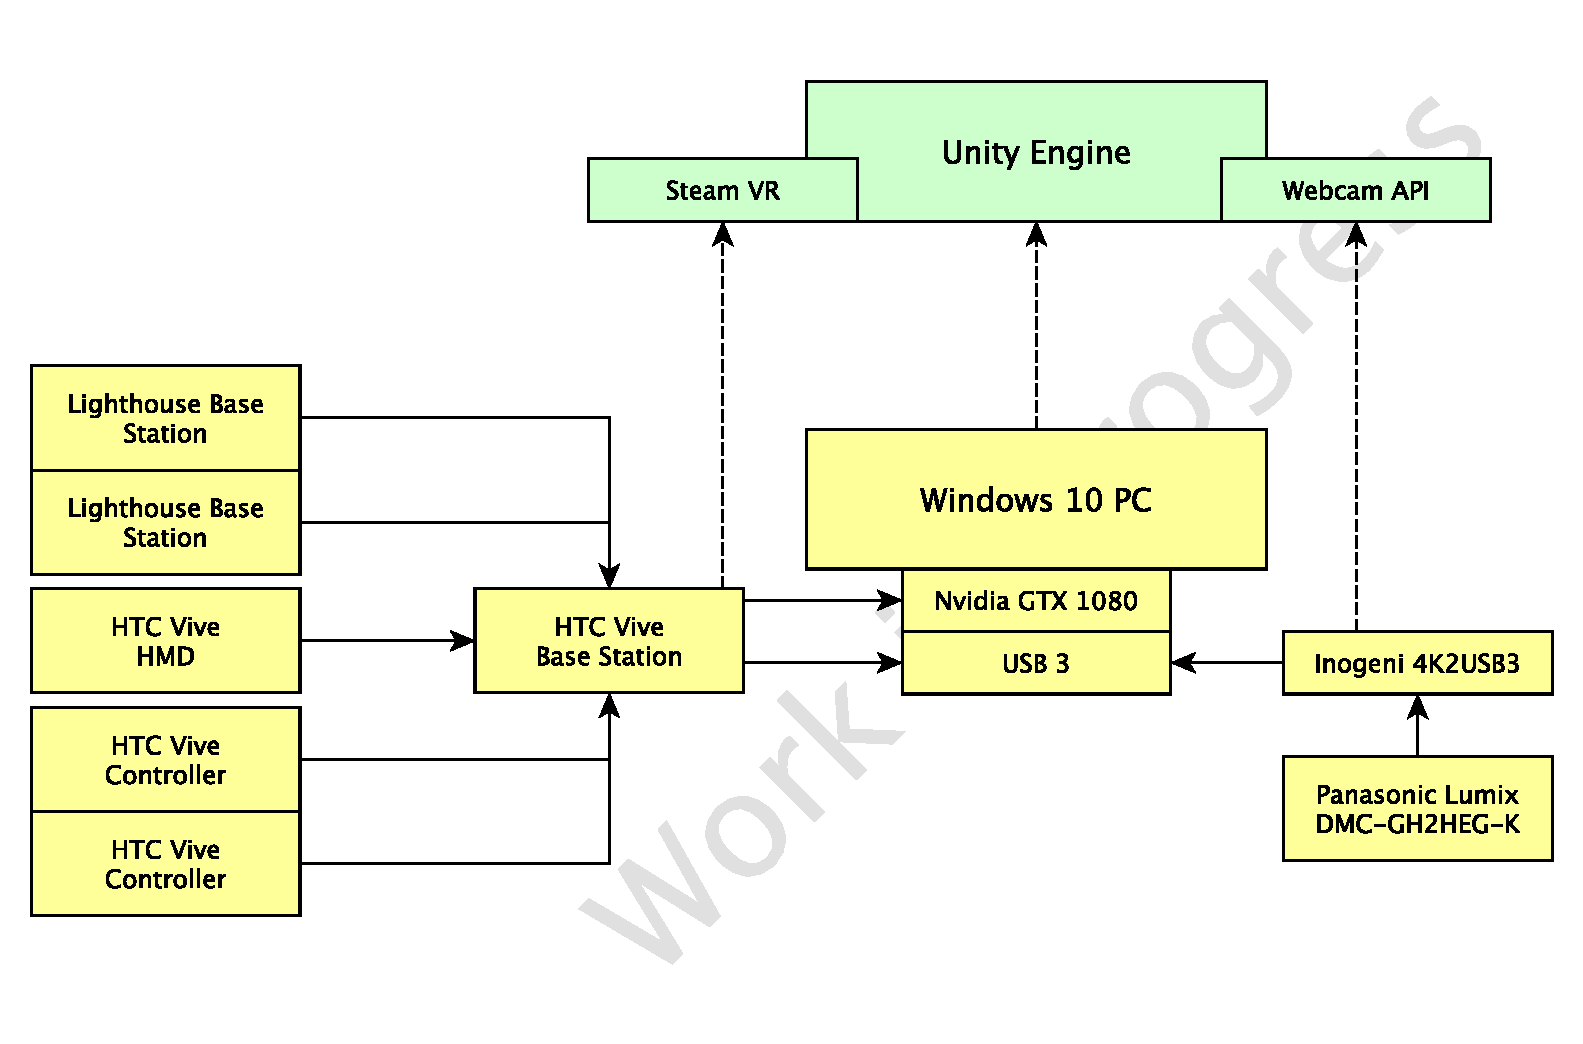
\includegraphics[width=\textwidth]{gfx/System-Components}
	\caption{Diagram of hard- and software components.}
	\label{fig:system-components}
\end{figure}

\section{Hardware Configuration}
\label{sec:hardware-config}

The hardware configuration is split in three main parts:
\begin{my_list}
	\item Windows PC Workstation
	\item Virtual Reality Tracking Solution
	\item Motion Video Input Feed
\end{my_list}

Each individual configuration is basically interchangeable with other systems, 
as long as predefined conditions are met. Each condition is listed first in 
each subsection.

\subsection{PC Workstation}

As the software is built in the Unity Engine, the workstation is limited to 
either Windows or Mac OS X systems the only requirement - besides being 
powerful enough to render the 3D scenes - is two USB3 ports to ensure enough 
data throughput for the video and virtual reality solution, as well as two 
video outputs for a monitor and its headset.
\newline
The configuration used for this thesis is:
\begin{lstlisting}
	CPU: Intel i7-6700 @ 3.40 GHz
	RAM: 16GB DDR4
	GPU: Nvidia Geforce GTX 1080
	System: Windows 10 v. 1703
	Engine: Unity 5.6f3
\end{lstlisting}

This system configuration is to date a high-end workstation that has an 
abundance of render performance and memory for complex and taxing computations 
that have to be performed for a mixed reality composition.

\subsection{Inogeni 4K2USB3 Capture Device}
The Ingoeni 4K2USB3 converter is a standalone box that allows to receive any 
HDMI source and converts it as a webcam video feed usable by "plug'n'play" 
device management of Windows. It's advantage is that it enables any HMDI source 
to be usable as system webcam, thus enabling and arbitrary choice of video 
cameras and a very simple integration with any software through the systems 
provided webcam API. With help of the converter box it's possible to request a 
webcam as video resource and process that video feed as a texture on the GPU.

\subsection{Panasonic GH2 System Camera}
This camera provides a direct video feed via HDMI with low latency. It can 
directly feed into the Inogeni 4K2USB3 and produces a stable, high quality 
video feed with a low signal to noise ratio in well lit environments. 
Additionally it has a well sized photo sensor allowing the camera to capture 
singular frames with reduced motion blur.

\subsection{HTC Vive with Controllers and Lighthouses}
The currently best virtual reality and tracking device available to the public 
is the HTC Vive. It includes two infrared sending stations called "Lighthouse", 
two Vive Controllers\footnote{often delightfully called "Wands" due to its 
controllers design} and a headset. Both, headset and controller systems, are 
enabled with 6 degrees of freedom (6DOF) tracking. The tracking system is a 
black box, in which only the transformation matrices for the hand controllers 
and the HMD can be accessed\footnote{as well as sensor input data from the 
controllers}, which already have been processed by the additional SteamVR 
software. By default this transformation has a normalized length of 1 unit to 1 
meter. Designing scenery and sense of size is therefore rather imaginable. The 
data provisioning is done by a library called "SteamVR for Unity", which makes 
the usage of said matrices in engine fully transparent.

\subsection{Vive Controller Tripod Mount}
Most cameras have a standardized way of mounting tripods. Since the Vive  
controllers have no reference plane. Minuscule differences in mounting angles 
change the projection parameters to noticeable effects, so it was necessary to 
build a mount for the camera to keep controller and video equipment 
transformation synchronized.

\begin{figure}[htb]
	\includegraphics[width=\textwidth]{gfx/system/mount.png}
	\caption{Camera mount for a HTC Vive controller, mounted on the cameras 
		tripod mount}
	\label{fig:system:camera-mount}
\end{figure}

I've built a mount that fits on tripod attachment points and keeps the 
controller locked in the same rotation and position (see figure 
\ref{fig:system:camera-mount}).



\section{Software}

The software of choice is Unity3D, which is a free game engine for students, 
non-profit organizations and small studios. It provides an easy introduction to 
game / 3D engine programming and has a huge development community. While it is 
not the technologically most advanced engine, its fairly easy usage and fast 
development cycles make it a great tool for a bachelor thesis.
\newline
Thankfully, the high abstraction of system APIs means that cross-platform 
development only needs a single code base and makes excruciating tasks like 
webcam access simple - so much so that it boils down to one line of code. 
However, this has drawbacks in overall performance, partially introduced by the 
engine's garbage collection, which are no issue for the used system.
\newline
Its weakness is usually API documentation and - on the downside, too - high 
abstraction levels from most APIs. For example, Unity relies on its own shading 
language which cross-compiles to HLSL, OpenGL and WebGL - this leads to 
problems in buffer and data management, which cannot be controlled well inside 
its render loop.

The software discussed in this thesis integrates and depends additionally on 
SteamVR, a library for Unity, providing the necessary tracking data in the 
engine. SteamVR is developed by Valve, the software is available for free on 
Steam, the complementary library is hosted on GitHub. As of writing this 
thesis, SteamVR is available for Windows and Mac OS X and the software of this 
thesis works on both systems. 

There are no further dependencies or external libraries used.
% !TEX root = ../thesis-example.tex
%
\chapter{From Video to Mixed Reality}
\label{chap:video2mr}

\todo[inline]{Needs better sourcing.}

To achieve a real time rendering environment, as previously mentioned, there 
are two main production cycles. The one discussed in this thesis resolves this 
problem by staying inside on application with multiple render cycles per frame. 
\newline
The first and foremost render cycle is the stereoscopic output of the Vive HMD, 
which has a set framerate of either 45 or 90 frames per second. It is important 
to have a consistent performance, otherwise the experience for the actor with 
the HMD will have a terrible experience.
\newline
The secondary render cycle has to be done on the same frame, which is a virtual 
camera inside the virtual scene and the relative position of the real world HMD 
and real world camera. Since the SteamVR library for the HTC Vive already 
exposes a normalized, synchronized tracking, it is easily possible to position 
the virtual camera at an accurate location.

The following chapter describes the techniques used to transform motion video 
inside a greenscreen into a mixed reality image. As brief overview, the steps 
required are performed in referential order from the motion video from the 
camera feed. This is different to the render order but gives a better 
understanding of the techniques used to achieve mixed reality imagery.

% !TeX spellcheck = en_US
% !TEX root = ../thesis-example.tex
%
\section{Chroma Key}
\label{sec:chromakey}

Beginning from a real-world camera, the video signal travels through the 
Inogeni 4KUSB3 converter and is accessible with the systems API for webcams. 
(See figure \ref{fig:system-components})

\begin{figure}[htb]
	\centering
	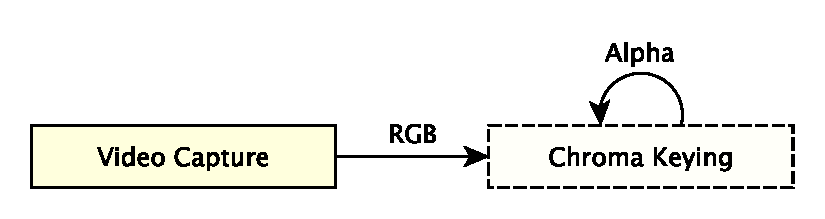
\includegraphics[width=.7\textwidth]{gfx/pipeline/4_1_chroma.pdf}
	\caption{Initial step upon receiving the camera image}
	\label{fig:steps:chroma}
\end{figure}

The initial step is to remove the green (or blue) background from the image, 
which should be live footage of a green (or blue) box. Other literature usually 
refers to it as "pulling a video matte" or "chroma keying." For a reference 
green, there has to be a color picked manually in the material editor of Unity 
--- this was made by a checkbox to show raw output from the camera (eg. fig. 
\ref{fig:chroma:editor}). Then an average green from the background box can be 
picked. This is an important setup step, since lightning situations can vary 
greatly and minor differences in light setups can have a great effect on the 
outcome of visible green background captured by the camera, thus making a 
recalibration necessary.

\begin{figure}[htb]
	\centering
	\includegraphics[width=.45\textwidth]{gfx/distances/material-editor.png}
	\caption{Material Editor inside Unity}
	\label{fig:chroma:editor}
\end{figure}

An extreme example case is used for comparing different chroma keying variants, 
which shows high motion blur due to a low shutter speed of the capturing 
camera and fast movement of the depicted actor:

\begin{figure}[htb]
	\includegraphics[width=\textwidth]{gfx/distances/example.png}
	\caption{Comparison Image \cite{vimeo:shia:2015} --- sRGB Output}
	\label{fig:chroma:color}
\end{figure}

\subsection{Initial Assumption}

Each RGB color can be represented as a discrete 3-Vector of (red, green and 
blue)  values in range of $[0, 1]$\footnote{Software RGBA color representations 
usually take 8bit per color channel and map between $[0, 255]$ --- graphic 
computing usually maps between $[0, 1]$}. An interpolation between two colors 
can be summarized as a matting equation as follows, where a foreground image 
$C_F$ and a background image $C_B - \alpha_B$ is assumed to be $1$:

\eq{eq:chroma:assumption:alpha:1}{
	I_{x, y} = \alpha_{x, y} C_{F_{x, y}} + (1 - \alpha_{x, y}) C_{B_{x, y}}
}

This matting equation has to be generalized for a later step, where 
$\protect\alpha$ is a value between [0, 1] on fore- and background, yielding a 
total Alpha of $\alpha_T$ as following:

\eq{eq:chroma:assumption:alpha:weak}{
	\alpha_T = \alpha_B * (1 - \alpha_F) \\
}

thus:

\eq{eq:chroma:assumption:alpha:cont}{
	I_{x, y} = (1 - \alpha_T) F_{x, y} + \alpha_T B{x, y}
}

This equation can take $\alpha_T < 1$ into account, which is needed later when 
fore- and background of the virtual environment are merged with a layer in 
between that results from the real world capture.

\subsection{Euclidean RGB Distance}
Assuming a source pixel color $C_S$ and a reference color $C_R$ we can 
calculate the euclidean distance between these two color vectors:
\eq{eq:euclidianrgb}{
	\alpha = \sqrt{(C_RR - C_SR)^2 + (C_RG - C_SG)^2 + (C_RB - C_SB)^2}
}

\begin{figure}[htb]
	\includegraphics[width=\textwidth]{gfx/distances/chroma-rgb.png}
	\caption{Chroma Keying by using euclidean RGB distance}
	\label{fig:chroma:euclidean:rgb}
\end{figure}

This is computationally very low cost and works well enough to detect a 
difference between two distinct colors. It fails to accommodate for coloring 
that is perceived as different, but tinted by the reference colors. Since the 
green screen material will never achieve 0\% reflectivity, some color will 
spill onto the filmed actor and will therefore generate unwanted chroma-keying 
artifacts, most noticeable on semi-glossy reflection of skin or color tints on 
white clothing.

\subsection{Euclidean YCgCo Distance}

YCgCo gets its name for Luminance (Y), chrominance green (Cg) and chrominance 
orange (Co) and helps decorrelating color spaces by splitting color-lightness 
from color chrominances, thus splicing the color model into brightness and 
color appearance. Since it is a fast, lossless color transformation it 
is used in example for H.264 video encoding and other image compression 
techniques. The two chrominance channels are then split into green to magenta 
and orange to blue color channels and allow for a more accurate distance 
calculation between two colors.

\begin{figure}[htb]
	\includegraphics[width=\textwidth]{gfx/distances/chroma-ycgco.png}
	\caption{Chroma Keying by using euclidean YCgCo distance}
	\label{fig:chroma:euclidean:ycgco}
\end{figure}

Transforming any RGB color to YCgCo can be done with a single matrix  
multiplication, which is --- again --- a very low-cost computation on a GPU:

\eq{eq:ycgco:transformation}{
	\begin{bmatrix}
		Y \\
		Cg \\
		Co \\
	\end{bmatrix}
	=
	\begin{bmatrix}
		 \frac{1}{4} && \frac{1}{2} &&  \frac{1}{4} \\
		-\frac{1}{4} && \frac{1}{2} && -\frac{1}{4} \\
		 \frac{1}{2} && 0           && -\frac{1}{2}
	\end{bmatrix}
	*
	\begin{bmatrix}
		R \\
		G \\
		B 
	\end{bmatrix}
}

Given two colors, one from the video source $C_S$ and a reference color $C_R$ 
it is now possible to calculate the euclidean distance on the two chrominance 
channels:

\eq{eq:ycgco:euclidean}{
	\alpha = \sqrt{(C_RCg - C_SCg)^2 + (C_RCo - C_SCo)^2}
}

Due to the increased decorrelation, the result is more accurate and shows less 
artifacts on target pixels, allowing for better matte pulling, less 
green edges and a more continuous, smooth image of an actor.

\subsection{Euclidean Lab Difference}
The International Color Consortium (ICC) defined 1976 \textit{Lab $\Delta$E} as 
a standard model of calculating color differences inside the \textit{Lab} color 
vector volume. The final distance calculation is a linear euclidean scalar as 
with all other models, but accommodates for perceived color differences. It is 
a more expensive computation and needs code branches, which will evaluate all 
branches first by the GPU before using either code path.

A reference white has to be used to convert RGB to the Lab color model to 
accommodate for different RGB color spaces\footnote{which are usually only 
different on stored image material like photos or video}. Luckily the given 
webcam signal defaults to sRGB D65 and does not need a configurable reference 
matrix based on a given color model to handle different RGB color standards.

sRGB conversion needs to be converted to linear RGB while respecting light 
energy per color channel, rather than relative, perceived color brightness: 

\eq{chroma:inversecompanding}{
	v \in \{r, g, b\} \land V \in \{R, G, B\}
}

where: 

\eq{chroma:inverseRGBcompanding}{
	v = \\
	\begin{cases}
		\frac{V}{12.92}                 & \quad \text{if } V \leq 0.0405 \\
		(\frac{V + 0.055}{1.055})^{2.4} & \quad \text{otherwise}
	\end{cases}
}

from there an linear RGB color can be converted to XYZ by the following 
equation:

\eq{chroma:conversioncalc}{
	\begin{bmatrix}
		X\\
		Y\\
		Z\\
	\end{bmatrix}
		=
	\begin{bmatrix}
		M
	\end{bmatrix}
	\begin{bmatrix}
		R\\
		G\\
		B\\
	\end{bmatrix}
}

where:

\eq{chroma:rgbmatrix}{
	\begin{bmatrix}
		M
	\end{bmatrix}
		=
	\begin{bmatrix}
		R X_r && G X_g && B X_b \\
		R Y_r && G Y_g && B Y_b \\
		R Z_r && G Z_g && B Z_b
	\end{bmatrix}
}


\eq{chroma:xyzmatrix}{
		\begin{bmatrix}
		X\\
		Y\\
		Z\\
	\end{bmatrix}
	\begin{bmatrix}
		M
	\end{bmatrix}
	=
	\begin{pmatrix}
		X_r / Y_r && X_g / Y_g && X_b / Y_g \\
		1 && 1 && 1 \\
		\frac{1-X_r-Y_r}{Y_r} && \frac{1-X_g-Y_g}{Y_g} && \frac{1-X_b-Y_b}{Y_b}
	\end{pmatrix}
}

The needed $\begin{bmatrix}M\end{bmatrix}$ for RGB D65 is defined as:

\eq{chroma:sRGBD65}{
	\begin{bmatrix}
		0.4124564 && 0.3575761 && 0.1804375 \\
		0.2126729 && 0.7151522 && 0.0721750 \\
		0.0193339 && 0.1191920 && 0.9503041 \\
	\end{bmatrix}
}

Based on a reference white $U_r \in \{X_r, Y_r, Z_r\}$:

\eq{chroma:xyz2lab:defines}{
	U \in \{X, Y, Z\} \land W \in \{L, a, b\}
}

\eq{chroma:xyz2lab:epsilon}{
	\epsilon = 0.008856 \land \kappa = 903.3
}

where:

\eq{chroma:xyz2lab:ref}{
	w_r = \frac{U}{U_r}
}

\eq{chroma:xyz2lab:channel}{
	f(w) = \\
	\begin{cases}
		\sqrt[3]{w_r}      & \quad \text{if } U > \epsilon \\
		\frac{\kappa w_r + 16}{116} & \quad \text{otherwise}
	\end{cases}
}


\eq{chroma:xyz2lab:conversion}{
	\begin{bmatrix}
		L \\
		a \\
		b \\
	\end{bmatrix}
	=
	\begin{bmatrix}
		116 f_y - 16 \\
		500 (f_x - f_y) \\
		200 (f_y - f_z)
	\end{bmatrix}
}

With this conversion from sRGB to linear RGB to XYZ to Lab we can now calculate 
the euclidian linear distance between two colors $C_S$ and $C_R$, which already 
have been converted to Lab:

\eq{chroma:cie76:distance}{
	\Delta E = \sqrt{(C_R L - C_S L)^2 + (C_R a - C_S a)^2 + (C_R b - C_S b)^2}
}

The resulting values are rated by their perceptive difference (after Mkrzycki 
et. al. \cite{mokrzycki:2012}):

\begin{tabular}[htb]{l | l}
	0.0 \dots 0.5 & the difference is unnoticeable \\
	0.5 \dots 1.0 & the difference is only noticed by an experienced observer \\
	1.0 \dots 2.0 & the difference is also noticed by an unexperienced observer 
	\\
	2.0 \dots 4.0 & the difference is clearly noticeable \\
	4.0 \dots 5.0 & fundamental color difference  \\
	> 5.0 		  & gives the impression that these are two different 
	colors
\end{tabular}

Now it's possible to map alpha values for each pixel based on $\Delta$E 
distances between $m, n$ by clamping and biasing $\Delta$E with a proposed 
"smooth step" algorithm:

\eq{chroma:cie76:clamp}{
	f({\Delta E}) = x = \frac{\Delta E - n}{m - n}
}

\eq{chroma:cie76:min/max}{
	g(f({\Delta E})) = y =
	\begin{cases}
		n        & \quad \text{if } x \leq n \\
		x        & \quad \text{if } n \leq x \leq m \\
		m        & \quad \text{if } m \leq x
	\end{cases}
}

\eq{chroma:cie76:mapping}{
	\alpha(I_{x, y}) = 3 y ^2 - 2 y ^3
}

With that we receive a more natural matte with nearly no green edges, 
continuous actor imagery and smooth alpha transition between actor and green 
screen. Motion blur is hard to account for and is even with professional video 
matting hardware, extensive post production or intrinsic frame matting 
algorithms hard to remove without rough image results.

\begin{figure}[htb]
	\includegraphics[width=\textwidth]{gfx/distances/chroma-deltae.png}
	\caption{Chroma Keying by using $\protect\Delta $E distance}
	\label{fig:chroma:deltae}
\end{figure}

\subsection{Comparison between Computational Models}

To chose the best variant, balancing runtime and efficiency, there has to be a 
comparison between the presented methods. Again, the previous image will be 
used, since it has complicated color mixing between background and actor. First 
we pick scan line of the image, in this case the 301st row from top, and 
calculate the color distance from each pixel to a reference color $[R, G, B] = 
[0.341, 0.588, 0.42]$.

As seen in figure \ref{fig:chroma:image_comparison}d, CIEDE76s performance is 
significantly better in separating colors and has a broader margin between 
green background and other foreground. This can be observed in figure 
\ref{fig:chroma:image_comparison}, where the scan line is set as background and 
the values are normalized again:

\begin{figure}[htbp]
	\caption{Comparison between different color distance methods}
	\label{fig:chroma:image_comparison}
	\begin{subfigure}[t]{.65\textwidth}
		\centering
		\includegraphics[width=\textwidth]{gfx/distances/color-rgb.png}
		\caption{RGB color distance} 
	\end{subfigure}
	\begin{subfigure}[t]{.3\textwidth}
		\centering
		\includegraphics[width=\textwidth]{gfx/distances/zoom-rgb.png}
	\end{subfigure}
	\begin{subfigure}[t]{.65\textwidth}
		\centering
		\includegraphics[width=\textwidth]{gfx/distances/color-ycgco.png}
		\caption{YCgCo color distance}
	\end{subfigure}
	\begin{subfigure}[t]{.3\textwidth}
		\centering
		\includegraphics[width=\textwidth]{gfx/distances/zoom-ycgco.png}
	\end{subfigure}
	\begin{subfigure}[t]{.65\textwidth}
		\centering
		\includegraphics[width=\textwidth]{gfx/distances/color-ciede76.png}
		\caption{CIEDE76 color distance}
	\end{subfigure}
	\begin{subfigure}[t]{.3\textwidth}
		\centering
		\includegraphics[width=\textwidth]{gfx/distances/zoom-delta_e.png}
	\end{subfigure}
	\begin{subfigure}[t]{\textwidth}
		\centering
		\includegraphics[width=\textwidth]{gfx/distances/dist-comp.png}
		\caption{Normalized graph comparing color difference methods}
	\end{subfigure}
	\begin{subfigure}[t]{\textwidth}
		\includegraphics[width=\textwidth]{gfx/distances/ciede-comp.png}
		\caption{Comparison with different CIEDE $\Delta E$ variants}
	\end{subfigure}
\end{figure}
Additionally, CIEDE76 shows less variance on similar colored spaces to the 
target color as well as high color difference peaks on all other pixels. This 
yields an accurate upper and lower limit, in which the green screen can be 
calibrated in.
\newline
Finally, comparing CIEDE76, CIEDE94 and CIEDE2000 reveals, that CIEDE76 
performs well enough while having the lowest performance overhead. The 
similarities between the 1976 and 2000 method are very apparent, while 
CIEDE2000 has a significantly more complex algorithm. (cf.  
\cite{sharma:ciede2000:2005}) Performing the same operation on the same data 
with different CIEDE color distance revisions (fig. 
\ref{fig:chroma:image_comparison}e), that there is little difference between 
CIEDE76 and CIEDE2000.   % Chroma Key Section
% !TeX spellcheck = en_US
% !TEX root = ../thesis-example.tex
%
\section{Camera Input Lag}

After the rather simple integration of the keyed video signal into the scene, 
where the 3D environment is used as background, an offset between the render 
image from the scene and captured footage from the camera can be observed due 
to the pipeline from the capturing device through video converting of the 
Inogeni 4KUSB3 bound to the systems webcam API.

\begin{figure}[htb]
	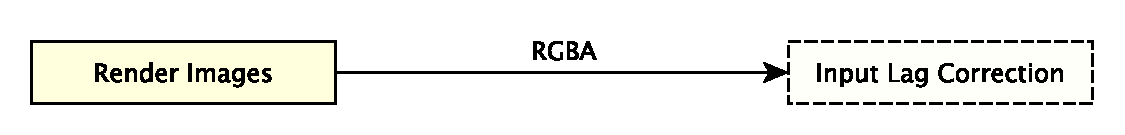
\includegraphics[width=\textwidth]{gfx/pipeline/4_2_swapper.pdf}
	\caption{The initial step upon receiving the camera image is to adjust the 
	time drift between engine renderings and video capture}
	\label{fig:steps:swapper}
\end{figure}

After consulting the specification of the Inogeni 4K2USB3 it states that a 
conversion from any HDMI video source takes two intrinsic frames for encoding. 
The camera framerate is $F_C = 25 \frac{frames}{second}$. This would mean, in 
theory:

\eq{offsets:timing:1}{
	t = \frac{2}{F_C}
}

Assuming 25 frames per second, that is $\frac{1}{30}s$:

\eq{offsets:timing:2}{
	t =  \frac{2}{25 \frac{frame}{second}}
}

\eq{offsets:timing:3}{
	t = 80ms
}

The observed offset from camera to engine is far longer in reality and remains 
at about 260ms after testing this setup and observing the drift, therefore 
seeing noticeable in any motion video as shown in figure 
\ref{fig:offsets:example}.

\begin{figure}[htbp]
	\caption[Aligned and unaligned frames]{Visual comparison between unaligned 
	and aligned frames\footnotemark}
	\label{fig:offsets:example}
	\begin{subfigure}[t]{.45\textwidth}
		\centering
		\includegraphics[width=\textwidth]{gfx/offsets/not_aligned.png}
		\caption{Before video and engine frames have been aligned, there is a 
		noticable difference in motion}
	\end{subfigure}
	\begin{subfigure}[t]{.45\textwidth}
		\centering
		\includegraphics[width=\textwidth]{gfx/offsets/aligned.png}
		\caption{After aligning frames the motion in engine and video capture 
		are in sync}
	\end{subfigure}
\end{figure}

\footnotetext{a video example is provided on the additional storage device}

To mitigate this offset there are two options:

\begin{my_list}
	\item Change the camera setup - for example a direct webcam, which 
	usually has a lower input latency, ranging between 5 - 250ms. That would 
	degrade the image quality significantly but would enable better rendering 
	conditions inside the engine.
	\item Capture virtual images of the 3D environment and keep them on the GPU 
	until a real world video frame is loaded onto the GPU for usage - assuming 
	that the time drift is constant. This keeps the image quality but needs 
	significant effort to reproduce the rendering conditions at the engine time 
	when a video frame was taken.
\end{my_list}

The proposed solution for this thesis uses the secondary option, since it is 
able to minimize any kind of constant offset between render image and a video 
stream, the hardware setup can stay dynamic\footnote{as long as it is provided 
by the systems webcam API} and it is little to no difference by switching to a 
webcam-integrated solution than an encoding box and the resulting displayed 
image has imperceptible differences to the former variant. It is therefore more 
user friendly and can accommodate for a wide range of video devices.

\begin{figure}[htb]
	\centering
	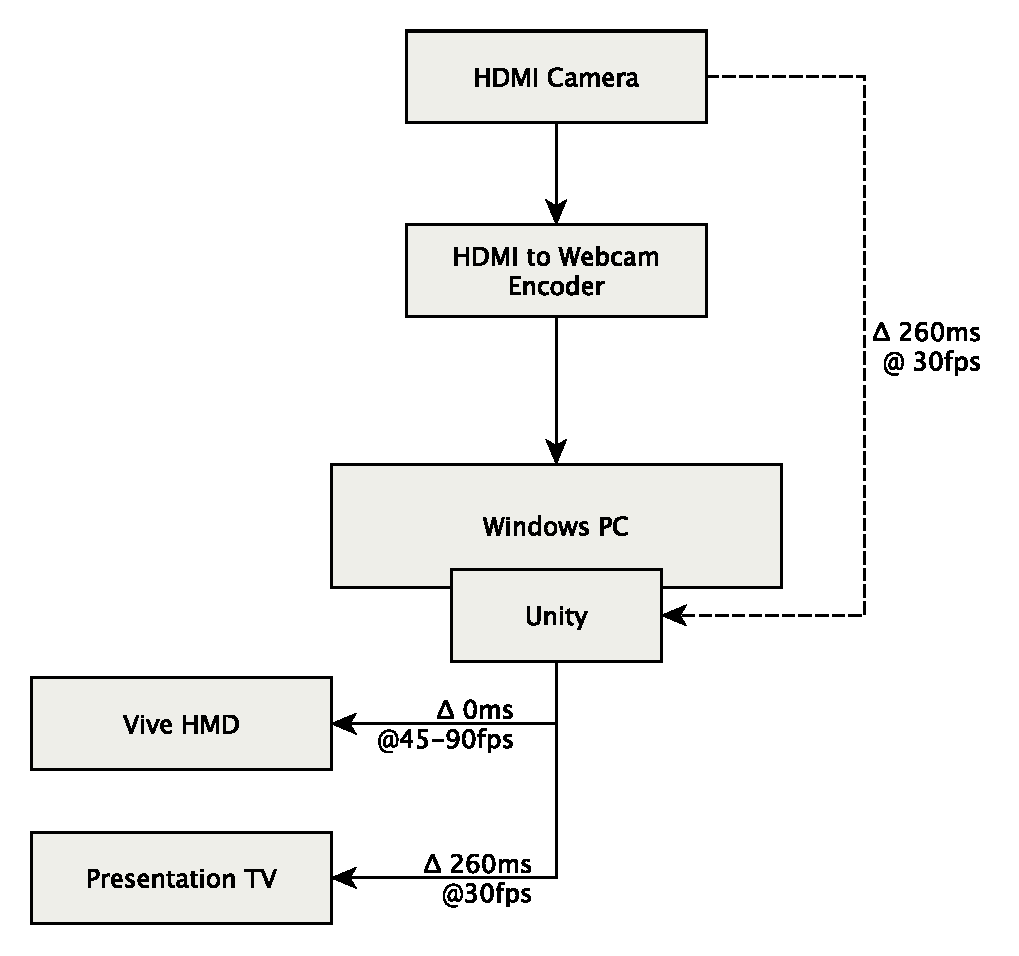
\includegraphics[width=.85\textwidth]{gfx/FPS-Timing-Components.pdf}
	\caption{Components in considering video input lag and frame rates. While 
	latencies between each components cannot measured, it is observed with help 
	of an interactive VR object.}
	\label{fig:offsets:components}
\end{figure}

Based on the component diagram \ref{fig:offsets:components} there are two 
important takeaways: 

\begin{my_list}
	\item There is an input latency between the production camera and the Unity 
	Engine, which in turn needs to be reproduced on the mixed reality 
	presenting device
	\item Frame rates between the Vive HMD and the presentation TV differ 
	because the TV's frame rate should be matched to the input video feed from 
	the camera (see section \ref{sec:framejitter})
\end{my_list}

At the time of writing Unity does not support dynamic frame rates on multiple 
viewports\footnote{A viewport can be either a D3D, OpenGL or Metal 3D context}.
\newline
It is possible to manually initiate a virtual camera's rendering, however, this 
causes the render loop to mistime and yields inconsistent frame timings inside 
the HMD and is no different between the average GPU load to display the 
presentation TV's viewport. It makes no perceptive difference if a scene 
renders 11ms twice and then falls down to 22ms once --- however the observed 
stuttering is a major degradation of the actors experience and often times 
causes motion sickness (fig. \ref{fig:cameralag:mistiming}).

\begin{figure}[htbp]
	\caption{Differences in performance based on rendering strategy}
	\label{fig:cameralag:mistiming}
	\begin{subfigure}[t]{\textwidth}
		\centering
		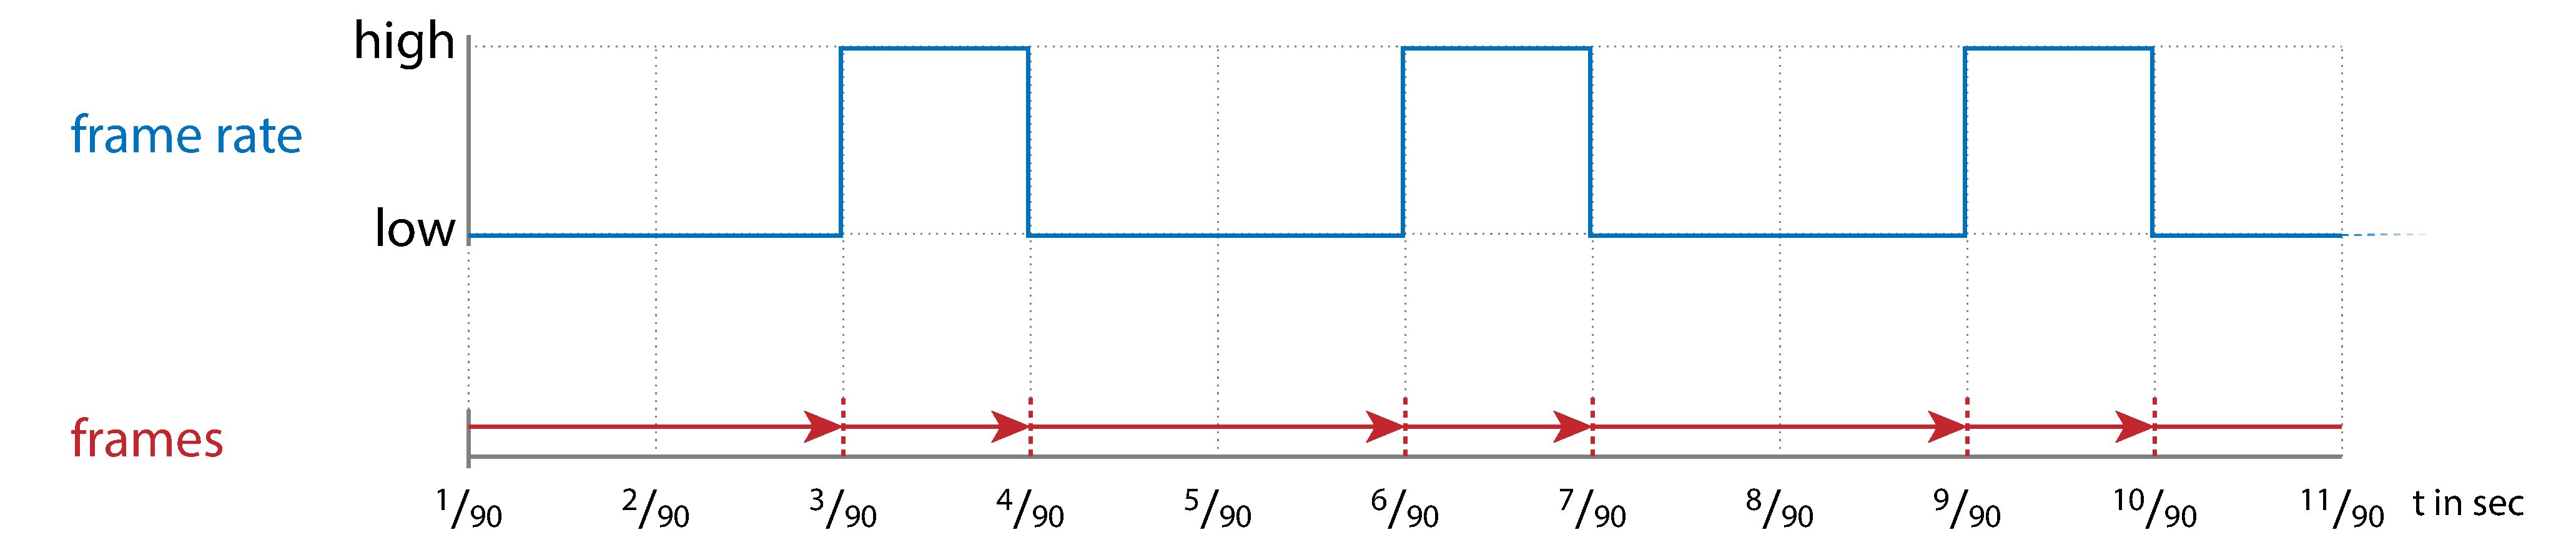
\includegraphics[width=\textwidth]{gfx/mistiming/variable.pdf}
		\caption{Initiating rendering when needed can cause stuttering 
		performance inside the headset, yielding motion sickness for the VR 
		actor}
	\end{subfigure}
	\begin{subfigure}[t]{\textwidth}
		\centering
		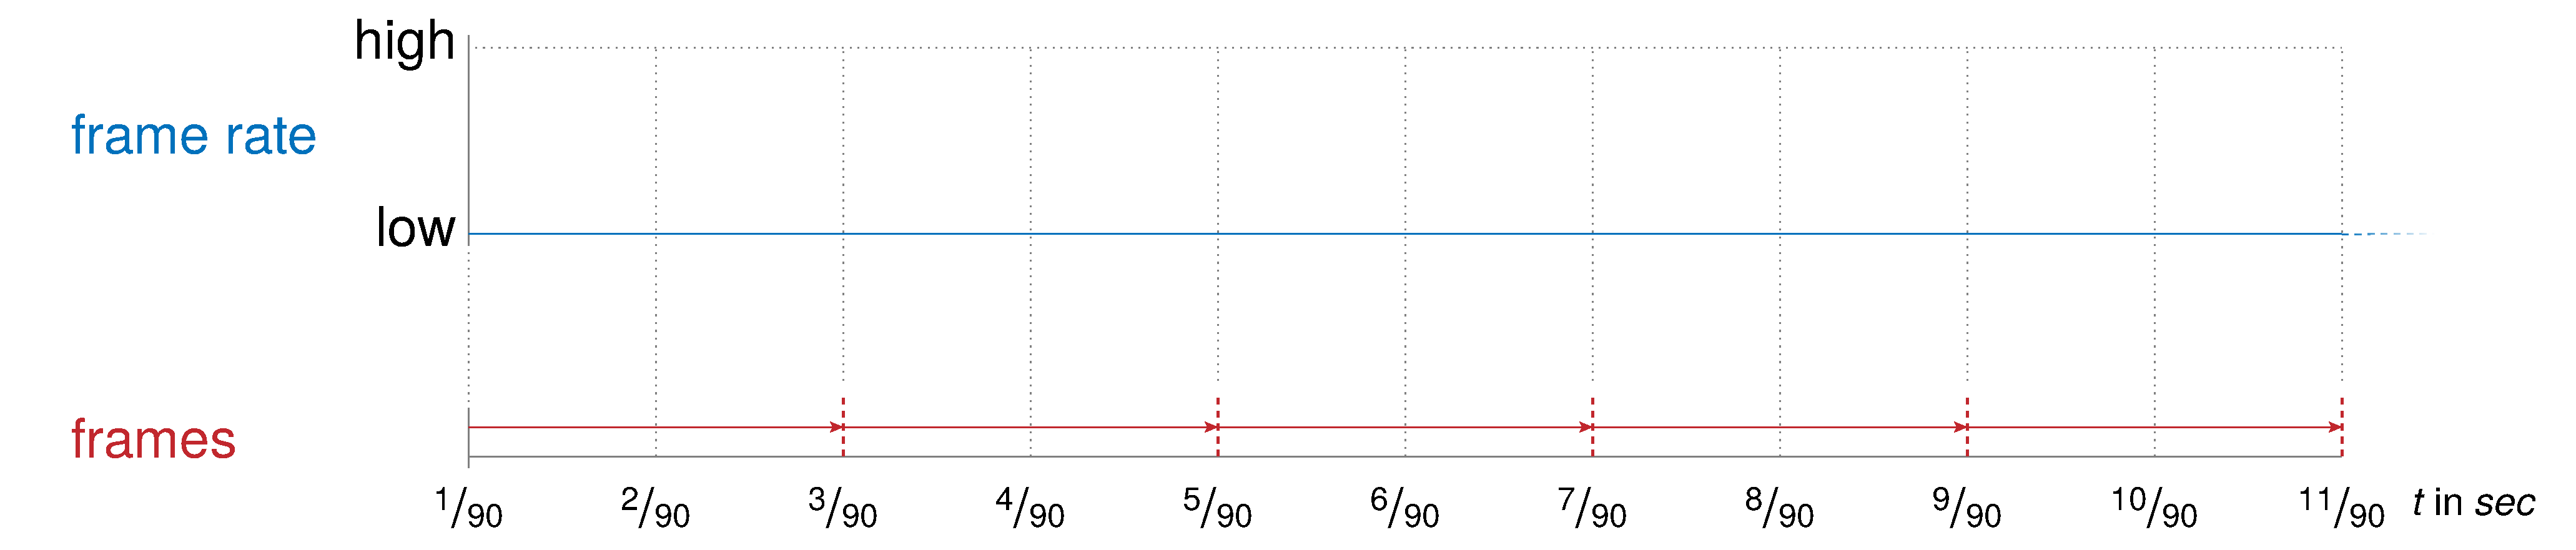
\includegraphics[width=\textwidth]{gfx/mistiming/stable.pdf}
		\caption{Consistent poor performance is less irritating for the VR 
		actor and makes no difference for a Mixed Reality composition}
	\end{subfigure}
\end{figure}

To conclude: The software has to store a set amount of \gls{framebuffer}s and 
cycle them at the right frame to guarantee minimal delays between camera and 3D 
environment, thus realigning the observed time drift between the engine and 
captured video frames.

Noteworthy is that the render loop can be 45 or 90 fps, depending on scene 
complexity, overall system performance or - especially in case of Unitys 
outdated C\# version - garbage collection, that could halt the engine for a 
significant amount of time. To account for this, a strategy is needed in which 
Unity's \code{Time.deltaTime} property is used, which describes the time 
between last and current frame, allowing for accurate timing how framebuffers 
have to be handled and swapped.

\subsection{Framebuffer Swapper Implementation}

Unity has a well engineered engine loop, where it can perform different 
operations at specific steps of the main engine execution\footnote{For more 
detail about Unity's core loop there is a flowchart in the Appendix 
\ref{app:engineloop}, depicting MonoBehaviors life cycle.}. As 
initial data needed is \code{cameraFPS}, \code{cameraOffset} and 
\code{Time.deltaTime}. With that input it is possible to calculate the 
\code{frameWindow}, which is the time of one displayed frame and 
\code{delay}, which is the time drift in frames between camera and engine:

\eq{eq:swapper:vars:1}{
	\textnormal{frameWindow} = \frac{1}{\textnormal{cameraFPS}}
}

\eq{eq:swapper:vars:2}{
	\textnormal{delay} =
		\frac{\textnormal{cameraOffset}}{\textnormal{frameWindow}}
}

\subsection{Double Access Ringbuffer}

In Unity's case a framebuffer is called \code{\gls{render texture}}. To spare 
memory and bandwidth overhead it is possible to reuse previously allocated 
\code{RenderTextures} by overwriting the second oldest \code{RenderTexture} and 
compositing a mixed reality image with the oldest \code{RenderTexture}(see  
figure \ref{fig:offsets:framesquashing}).

\begin{figure}[ht]
	\centering
	\includegraphics[width=.5\textwidth]{gfx/ringbuffer_schematics.png}
	\caption{Schema of an the ringbuffer}
	\label{fig:offsets:ringbuffer}
\end{figure}

To accommodate for that behavior we have to write frame data into the current 
index and display the frame on its next index. After that step is taken we 
increment by one. This way we’re overwriting the oldest seen 
\code{RenderTexture} and show the one written to the next index. A reference 
implementation can be found in appendix \ref{app:darbi}. % Render Buffer Swapper
% \input{content/chapter-concepts} % INCLUDE: concepts
% % !TeX spellcheck = en_US
% !TEX root = ../thesis-example.tex
%
\chapter{Outlook}

Motion capturing solution usually support a live preview of the actors motion 
inside a 3D environment - integrating an actor into a virtual world is not only 
in interest of VR developers, but motion video productions, too. Mixed Reality 
is an increasingly important topic for VR experiences. The number of MR-enabled 
or MR-captured software is increasing, likely due to the natural way of 
producing video material and easily understandable usage context of that 
software. Since stereo-rendering already requires the GPU to do multiple 
context switches per frame, future hardware will probably improve on that 
matter, enabling better performance for a complex Mixed Reality pipelines.

\section{Rendering Setup Variations}

There are a few approaches that work similarly, but differ with respect to 
complexity, their capabilities and hardware requirements. They have been 
already explored by producing companies and are covered here for completeness.

\subsection{Single Camera - 3D Plane in Space}

A novel approach is rendering the camera image onto a 2D plane positioned 
inside the 3D scene. This gives high control over projection parameters inside 
the engine without a running software and has good visual feedback for artists. 
All additional steps previously discussed are invalid, since this render can 
take full advantage of all runtime rendering parameters - which in turn means 
for lower render overhead and better graphical performance. It fails however on 
delay mitigation, which makes time drift between engine and camera visible, 
thus only usable with low latency video capturing devices (figure 
\ref{fig:alt-render:single-camera}).

\begin{figure}[htb]
	\includegraphics[width=\textwidth]{gfx/eval/plane-scene.png}
	\caption{Demonstrative scene with a plane at camera's rendering position}
	\label{fig:alt-render:single-camera}
\end{figure}

\subsection{Deferred Shading Path}

Similarly to the single camera approach, a deferred shader could be used, in 
which the plane is projected and texturized after the scene has rendered and 
the graphics buffer is still present - this way the total time taken for 
rendering can be calculated and the chroma keying step can be chosen for a 
faster variant if needed. This gives generally better control and could yield 
higher performance, since all projected fragments have an assigned depth - the 
camera image only has to be calculated where the actor's depth is smaller than 
the scenery's depth. This method is also lacking a way of adjusting for time 
drift. Additionally, calculating lightning is relatively expensive, due to the 
reprojection of lighting parameters inside the graphics buffer. A snapshot of 
this buffer cannot be stored - which is a limitation of Unity's render pipeline 
- and is lost after the rendering loop is completed.

\subsection{Composition Workstation}

Lastly, for full video production setups another rendering approach has been 
suggested, which has been used for the initial promo material for the HTC 
Vive\cite{valve:vive-trailer:2016}. It includes rendering a 4K video signal, 
outputting it to a composition PC which then takes care about managing time 
drift and video input from the camera.
\newline
The general concept involves a production of four 1920x1080 video signals of 
the virtual environment:
\begin{my_list}
	\item Background
	\item Foreground with blue matte
	\item Composite image
	\item First person view
\end{my_list}

\begin{figure}[htb]
	\includegraphics[width=\textwidth]{_external/media/4patch.jpg}
	\caption{4 Patch output for post / second station 
		production\cite{gartner:mixed-reality:2017}.}
	\label{fig:alt-render:4patch}
\end{figure}

Due to the system separation it is now possible to use green screen hardware 
compositors which have a visually higher quality in pulling the green 
background matte and then compositing it similarly into a mixed reality image. 
While this lifts some rendering overhead from the host PC, it fails in 
recreating a lightning environment for the VR actor and relies on two systems. 
While engine programming complexity decreases, operational setup complexity 
increases.

\section{Rendering Operational Variations}

This setup can handle another operational context by leaving out 
background-sorting and only rendering a virtual "front", by which a high 
quality augmented camera system can be achieved. Since time drift between 
camera and engine is already handled, it is possible to render an augmented 
image. Since depth information is lost, it is not possible to handle 
obstructions - for example by an interacting user that is standing in front of 
the augmented object. However, with some composition and choreography, AR 
footage can be showed and captured in live production for further use. A 
reference plane has to be used, either by a Vive Tracker\footnote{like a 
controller} or with feature markers.
\newline
This thesis assumes that the motion video feed is calibrated for a D65 white 
and augmented reality scenarios usually do not take real-world lightning into 
account, it would give a good natural and high quality look into augmented 
reality use cases.

\section{Multi User Augmented Reality}

While working with this setup another possible use-case showed up: On June 2017 
Apple presented their native Augmented Reality kit integrated in their consumer 
devices. Thus a similar system could be used to send all tracking parameters 
from the HTC Vive headset to these devices and have a calibrated north-wall 
with additional feature markers. This would potentially allow to have an 
augmented reality view around the actors world with a fast approximated actor 
position. It could then be possible for multiple users to use these devices as 
window into the virtual reality experience without a green screen at all. % INCLUDE: conclusion
\cleardoublepage

\begin{appendix}
	\printglossary[type=\acronymtype]
	
	\printglossary[type=main]
	\cleardoublepage
\end{appendix}


% --------------------------
% Back matter
% --------------------------
{%
\setstretch{1.1}
\renewcommand{\bibfont}{\normalfont\small}
\setlength{\biblabelsep}{0pt}
\setlength{\bibitemsep}{0.5\baselineskip plus 0.5\baselineskip}
\printbibliography[nottype=online]
\printbibliography[heading=subbibliography,title={Websites},type=online,prefixnumbers={@}]
}
\cleardoublepage

\listoffigures
\cleardoublepage

\listoftables
\cleardoublepage

\input{content/colophon}
\cleardoublepage

% !TEX root = ../thesis-example.tex
%
%************************************************
% Declaration
%************************************************
\pdfbookmark[0]{Declaration}{Declaration}
\chapter*{Declaration}
\label{sec:declaration}
\thispagestyle{empty}

Hereby I affirm that this thesis is written by myself and I have not used any 
additional resources or utilities.

\begin{center}
	\hrulefill
\end{center}

Hiermit versichere ich, dass meine Abschlussarbeit selbstständig verfasst und 
keine anderen als die angegebenen Quellen und Hilfsmittel benutzt habe.

\bigskip

\noindent\textit{\thesisUniversityCity, \thesisDate}

\smallskip

\begin{flushright}
	\begin{minipage}{5cm}
		\rule{\textwidth}{1pt}
		\centering\thesisName
	\end{minipage}
\end{flushright}

%*****************************************
%*****************************************

\clearpage
\newpage
\mbox{}

% **************************************************
% End of Document CONTENT
% **************************************************
\end{document}
